\documentclass[12pt]{article}
\usepackage[utf8]{inputenc}

\usepackage{lmodern}

\usepackage{enumitem}
\usepackage[margin=2cm]{geometry}

\usepackage{amsmath, amsfonts, amssymb}
\usepackage{graphicx}
%\usepackage{subfigure}
\usepackage{tikz}
\usepackage{pgfplots}
\usepackage{multicol}

\usepackage{comment}
\usepackage{url}
\usepackage{calc}
\usepackage{subcaption}
\usepackage[indent=0pt]{parskip}
\usepackage{animate}

\usepackage{array}
\usepackage{blkarray,booktabs, bigstrut}
\usepackage{bigints}

\pgfplotsset{compat=1.16}

% MATH commands
\newcommand{\ga}{\left\langle}
\newcommand{\da}{\right\rangle}
\newcommand{\oa}{\left\lbrace}
\newcommand{\fa}{\right\rbrace}
\newcommand{\oc}{\left[}
\newcommand{\fc}{\right]}
\newcommand{\op}{\left(}
\newcommand{\fp}{\right)}

\newcommand{\bi}{\mathbf{i}}
\newcommand{\bj}{\mathbf{j}}
\newcommand{\bk}{\mathbf{k}}
\newcommand{\bF}{\mathbf{F}}

\newcommand{\mR}{\mathbb{R}}

\newcommand{\ra}{\rightarrow}
\newcommand{\Ra}{\Rightarrow}

\newcommand{\sech}{\mathrm{sech}\,}
\newcommand{\csch}{\mathrm{csch}\,}
\newcommand{\curl}{\mathrm{curl}\,}
\newcommand{\dive}{\mathrm{div}\,}

\newcommand{\ve}{\varepsilon}
\newcommand{\spc}{\vspace*{0.5cm}}

\DeclareMathOperator{\Ran}{Ran}
\DeclareMathOperator{\Dom}{Dom}

\newcommand{\exo}[1]{\noindent\textcolor{red}{\fbox{\textbf{Problem {#1}}}\hrulefill}\\}
\newcommand{\qu}[4]{\noindent\textcolor{#4}{\fbox{\textbf{Section {#1} | Problem {#2}}} \hrulefill{{\fbox{\textbf{{#3} Points}}}}\\}}

\newcommand{\semester}{Spring 2023}

\newcommand{\CVup}{%

\begin{tikzpicture}
\draw[black, <->, >=latex] (-0.33, 0.5) .. controls (-0.125, 0) and (0.125, 0) .. (0.33, 0.5);
\end{tikzpicture}}

\newcommand{\CVupInc}{%
\begin{tikzpicture}
\draw[black, ->, >=latex] (0,0) .. controls (0.2, 0) and (0.4, 0.2) .. (0.5, 0.5);
\end{tikzpicture}}

\newcommand{\CVupDec}{%
\begin{tikzpicture}[rotate=270]
\draw[black, ->, >=latex] (0,0) .. controls (0.2, 0) and (0.4, 0.2) .. (0.5, 0.5);
\end{tikzpicture}}

\newcommand{\CVdown}{%
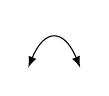
\begin{tikzpicture}
\draw[black, <->, >=latex] (-0.33, -0.5) .. controls (-0.125, 0) and (0.125, 0) .. (0.33, -0.5);
\end{tikzpicture}}

\newcommand{\CVdownInc}{%
\begin{tikzpicture}
\draw[black, ->, >=latex] (-0.5, -0.5) .. controls (-0.5, -0.3) and (-0.5, -0.1) .. (0,0);
\end{tikzpicture}}

\newcommand{\CVdownDec}{%
\begin{tikzpicture}[rotate=-90]
\draw[black, ->, >=latex] (-0.5, -0.5) .. controls (-0.5, -0.3) and (-0.5, -0.1) .. (0,0);
\end{tikzpicture}}

\begin{document}
	\noindent \hrulefill \\
	MATH-241 \hfill Pierre-Olivier Paris{\'e}\\
	Solutions Section 3-1 \hfill \semester \\\vspace*{-1cm}
	
	\noindent\hrulefill
	
	\spc
	
	\exo{30}
	\\
	The derivative is $f'(x) = 3x^2 + 12x - 15$. So the critical numbers are the solutions to the equation $x^2 + 4x -5= 0$. The solutions are $x = 1$ and $x = -5$. So, the critical numbers are $x = 1$ and $x = -5$ (the derivative exists everywhere).
	
	\spc
	
	\exo{34}
	\\
	The function is not differentiable at $c = 4/3$ because $g$ has a corner there. Therefore $c = 4/3$ is a critical point. 
	
	Now, for $t < 4/3$, we have that $3t - 4 < 0$ and
		\begin{align*}
		g(t) = -(3t - 4) = 4 - 3t .
		\end{align*}
	We have $g'(t) = -3$ and the number $-3$ is never zero. So no critical point for $t < 4/3$.
	
	Now, for $t > 4/3$, we have that $3t - 4 > 0$ and
		\begin{align*}
		g(t) = 3t - 4 .
		\end{align*}
	We have $g'(t) = 3$ and the number $3$ is never zero. So, no critical point for $t > 4/3$. 
	
	In summary, there is only one critical number at $c = 4/3$. 
	
	\spc
	
	\exo{38}
	\\
	The derivative of $g$ is
		\begin{align*}
		g'(x) = -\frac{2}{3} \frac{x}{(4 - x^2)^{2/3}} .
		\end{align*}
		
	The derivative does not exist when the denominator is zero. The denominator is zero if
		\begin{align*}
		4 - x^2 = 0 \iff x = \pm 2 .
		\end{align*}
	
	The derivative is zero if the numerator of $g'$ is zero. The numerator is zero if $x = 0$. 
	
	Therefore, the critical points are $c = -2$, $c = 0$, and $c = 2$. 
	
	\spc
	
	\exo{50}
	\\
	The derivative of the function is $f'(t) = 6t (t^2 - 4)^3$. So the critical points within $(-2, 3)$ are $t = 0$ and $t = 2$. 
	
	We have $f(-2) = 0$, $f(0) = -64$, $f(2) = 0$, and $f(3) = 125$. So the maximum is
		\begin{align*}
		M = 125
		\end{align*}
	and the minimum is
		\begin{align*}
		m = -64 .
		\end{align*}
	
	\spc
	
	\exo{52}
	\\
	The derivative of $f$ is
		\begin{align*}
		f'(x) = \frac{(x^2 - x + 1) - x (2x - 1)}{(x^2 - x + 1)^2} = \frac{-x^2 + 1}{(x^2 - x + 1)^2} = - \frac{1 - x^2}{(x^2 - x + 1)^2} .
		\end{align*}
	
	The critical points of $f$ are
		\begin{itemize}
		\item When $f'(x)$ does not exists. The denominator is zero if
			\begin{align*}
			x^2 -x + 1 = 0 .
			\end{align*}
		The discrimant of this quadratic is
			\begin{align*}
			b^2 - 4ac = 1 - 4 = -3 .
			\end{align*}
		Since the discrimant is negative, the expression $x^2 - x + 1$ is never zero.
		\item When $f'(x)$ is zero. The derivative $f'$ is zero if
			\begin{align*}
			1- x^2 = 0 \iff x = \pm 1 .
			\end{align*}
		\end{itemize}
	The critical points of $f$ are therefore $c = -1$ and $c = 1$. 
	
	Using the closed interval method, one critical point is within the interval $[0, 3]$. Therefore, we have
		\begin{align*}
		\max f(x) = \max \{ f(0) , f(1) , f (3) \} = \max \{ 0 , 1 , 3/7 \} = 1 .
		\end{align*}
		
	\spc
	
	\exo{54}
	\\
	We have to find the critical points inside the interval $(0, 2)$. The derivative of $f$ is
		\begin{align*}
		f'(t) = \frac{(1 + t^2)/2\sqrt{t} - \sqrt{t} (2t)}{(1 + t^2)^2} = \frac{1 + t^2 - 4t^2}{2 \sqrt{t} (1 + t^2)^2} = \frac{1 - 3t^2}{2 \sqrt{t} (1 + t^2)^2} .
		\end{align*}
	The zeros of the derivative are at $t = \pm \sqrt{1/3}$. We have to discard $-\sqrt{1/3}$ because it's not in the interval. The derivative exists at every point in $(0, 2)$. 
	
	Now the maximum and the minimum will be given by the max of the values $f(0) = 0$, $f(\sqrt{1/3}) \approx 0.5698$, and $f(2) \approx 0.2828$. So the maximum 
		\begin{align*}
		M = 0.5698
		\end{align*}
	and the minimum
		\begin{align*}
		m = 0.2828 .
		\end{align*}
	
	
\end{document}